\chapter{Testes}


Os testes foram concebidos de modo a englobar pequenas histórias de
uso, de um lado, e funcionalidades, de outro.

Os testes planejados de carga e salvamento de progresso foram suprimidos do projeto em razão de sua baixa prioridade quando comparados aos demais testes.

\section{Diálogos}

Este teste envolveu diversos subsistemas do projeto simultaneamente. não apenas o mecanismo de exibição de diálogo, como também o funcionamento da sequência do script de diálogo e as mudanças de crenças dos agentes do BDI foram testados conjuntamente. Estes sistemas haviam sido testados por si, independentemente, mas optou-se por apresentar neste documento uma pequena quantidade de testes significativos da correta operação dos sistemas.

\section{Navegação pelo jogo}

O teste de navegação incluiu a escolha das diferentes opções em cada uma das telas do jogo.

\section{Cenas}

Analogamente aos diálogos, foram testadas diversas cenas do jogo, embora nem todas sejam de fato parte integrante de sua versão final. Os testes ``extras'' tiveram por objetivo testar as funcionalidades implementada da linguagem script de cenas. (Nem todos os comandos previstos são usados nas cenas de fato produzidas para demonstração do projeto.)

\section{BDI em ação}
Este teste foi efeuado juntamente com um teste de diálogos. A ferramenta Jason oferece um recurso de monitoramento da base de crenças e intenções do agente o \emph{Jason Mind Inspector}(figura \ref{debug}), com tal recurso fomos capazes de apresentar todas as alterações que ocorreram nessa base durante um diálogo.
\begin{figure}
\centering
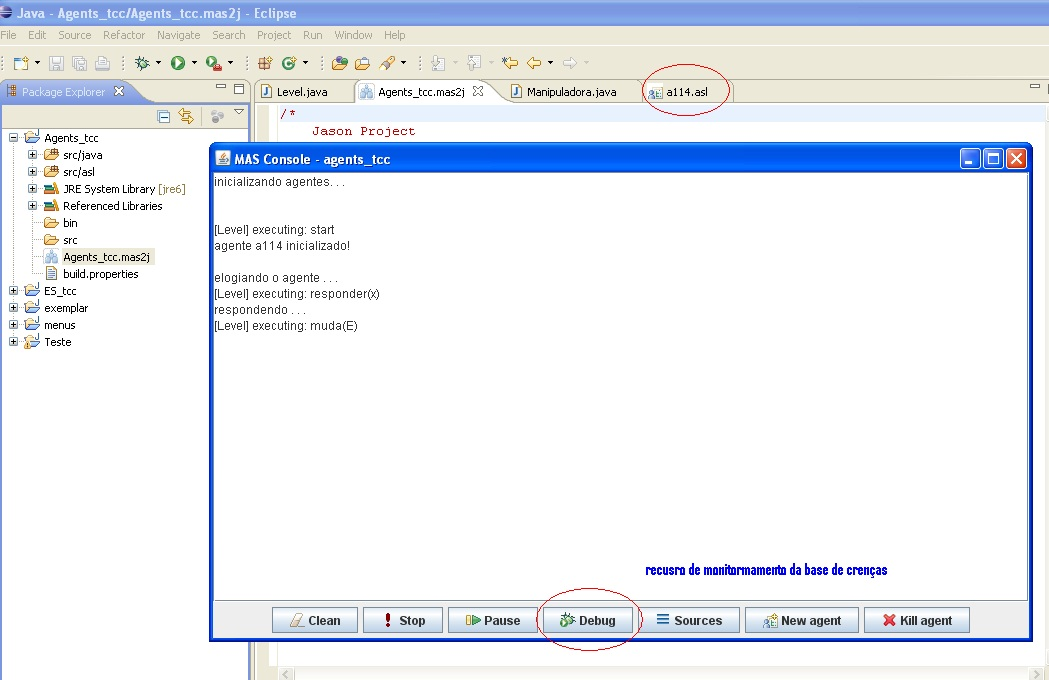
\includegraphics [height=10cm]{figuras/rodando_elogio_jose.jpg}
\caption{Recurso de monitoramento da base de crenças de agentes}
\label{debug}
\end{figure}

A seguir apresentamos uma pequena demonstração de como o agente altera seu estado psicológico em função de um estímulo.
Temos um agente do tipo civil, cuja personalidade foi definida como simpático e o estado psicológico foi definido como feliz, este agente recebeu um estímulo do tipo elogio, como era de se esperar, um agente simpático e feliz continuou simpático e ficou lisonjeado. Apresentamos abaixo o arquivo de modelo do agente antes (figura \ref{ze_antes}) e depois do elogio (figura \ref{ze_depois}) bem como sua base de crenças quando foi elogiado (figura \ref{base_crencas}).

\begin{figure}
\centering
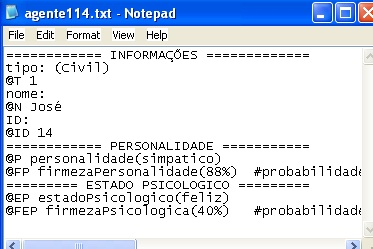
\includegraphics [height=10cm]{figuras/jose_antes.jpg}
\caption{Arquivo de modelo do agente antes do estimulo}
\label{ze_antes}
\end{figure}

\begin{figure}
\centering
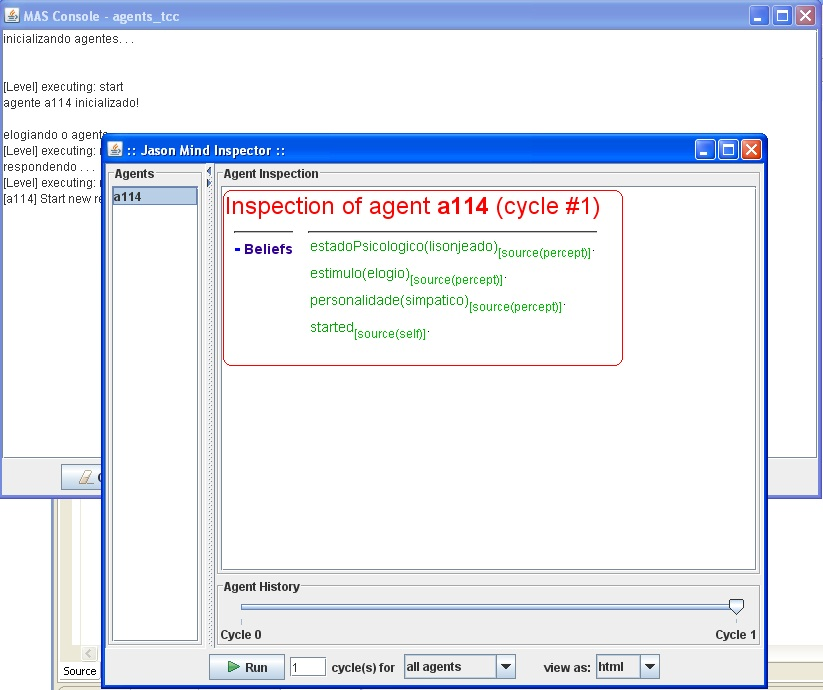
\includegraphics [height=10cm]{figuras/base_crencas_jose.jpg}
\caption{Base de crenças do agente no momento do estímulo}
\label{base_crencas}
\end{figure}

\begin{figure}
\centering
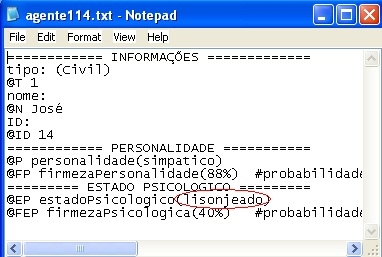
\includegraphics [height=10cm]{figuras/jose_depois.jpg}
\caption{Arquivo de modelo do agente depois do estimulo}
\label{ze_depois}
\end{figure}


\section{Inferência pelo Blackboard}
Da mesma forma que o teste anterior, utilizando o recurso de monitoração da base de crenças dos agentes (\emph{Jason Mind Inspector}), observamos o que aconteceu na base dos agentes ocultos quando uma informação foi adicionada por um agente policial.
Como foi explicado no capítulo anterior, existem agentes ocultos da polícia que fazem o processamento das informações enviadas peloas agentes policiais. As informações podem ser dos seguintes tipos (onde P~=~pessoa e L~=~lugar):
\begin{itemize}
\item P fez compra suspeita
\item P agiu de modo suspeito em L
\item L foi roubado com sucesso
\item L foi roubado sem sucesso
\end{itemize}
Quando um policial envia alguma das informações acima, ela é repassada a todos os agentes ocultos, no entanto, só alguns sabem processar a informação e geram novas informações que somente outros sabem processar e este processo continua até uma ou mais ações policiais serem geradas.
Dentre as ações que podem ser geradas temos:
\begin{itemize}
\item aumentar nivel suspeita de P
\item diminuir nivel suspeita de P
\item prender P
\item aumentar nivel segurança de L
\item diminuir nivel segurança L 
\end{itemize}
No teste realizado, um capanga (o agente a301) realizou uma atividade suspeita no banco. Um policial reportou aos agentes ocultos estas informações, e o agente oculto (policial) a251 concluiu que o nível de suspeita do capanga deveria ser aumentado e o agente oculto (policial) a252 concluiu que o nível de segurança do banco deveria ser aumentado, além disso, o nível de suspeita do capanga chegou em um nível tão alto que o agente oculto (policial) a255 decidiu decretar sua prisão.
Na figura \ref{blackB} temos a saída do programa para esta situação em termos das ações doas agentes.

\begin{figure}
\centering
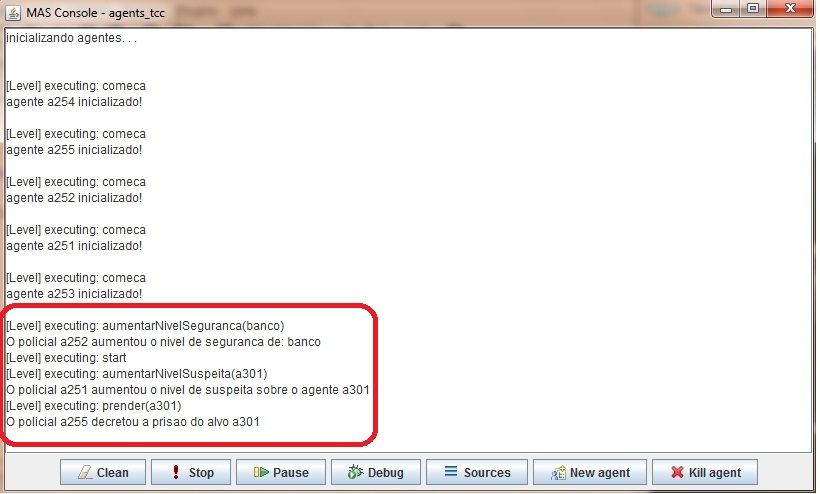
\includegraphics [height=10cm]{figuras/blackboard.jpg}
\caption{Demonstração do trabalho cooperativo entre os agentes da polícia}
\label{blackB}
\end{figure}

As ilustrações a seguir (\ref{baseA251},\ref{baseA252},\ref{baseA253},\ref{baseA254},\ref{baseA255})apresentam a base de crenças de cada agente, que conforme explicado deverá ser a mesma para todos os agentes. O fato de todos os agentes possuirem as mesmas crenças (as mesmas infromações), porém só alguns conseguem processá-las e gerar novas crenças para todos os outros agentes (novas informações), de forma a chegarem a uma ação da poícia é a aplicação clara da técnica blackboard, diversos agentes trabalhando cooperativamente transformando a infromação de entrada em ações de saída.

\begin{figure}
\centering
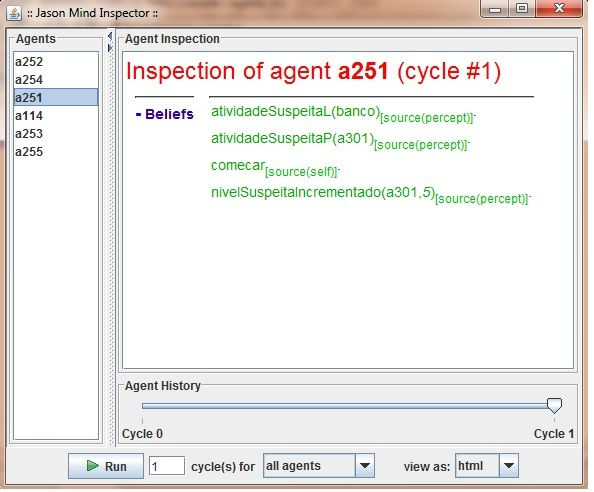
\includegraphics [height=10cm]{figuras/crencas_policial251.jpg}
\caption{Base de cranças do agente policial oculto a251}
\label{baseA251}
\end{figure}
\begin{figure}
\centering
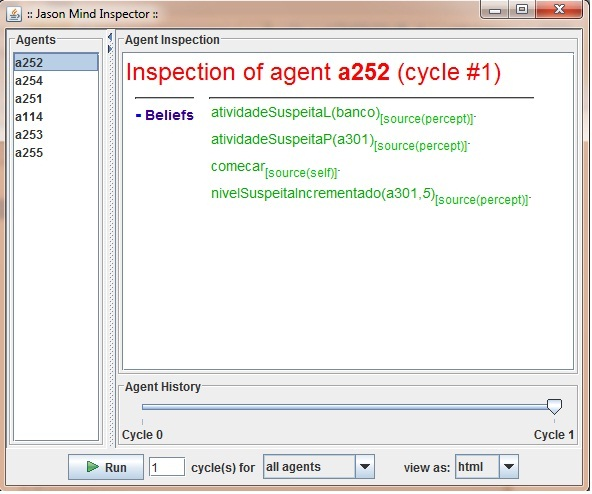
\includegraphics [height=10cm]{figuras/crencas_policial252.jpg}
\caption{Base de cranças do agente policial oculto a252}
\label{baseA252}
\end{figure}
\begin{figure}
\centering
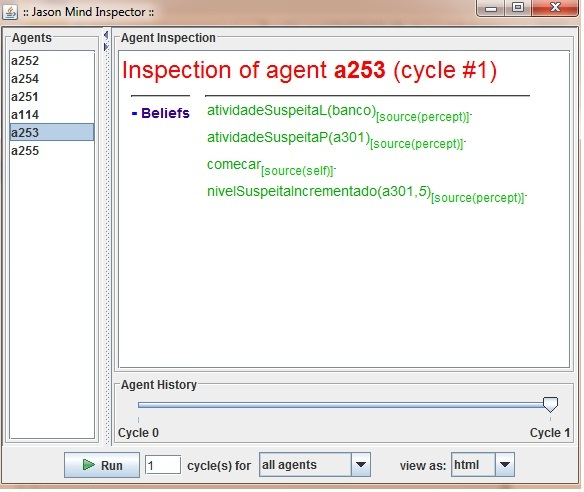
\includegraphics [height=10cm]{figuras/crencas_policial253.jpg}
\caption{Base de cranças do agente policial oculto a253}
\label{baseA253}
\end{figure}
\begin{figure}
\centering
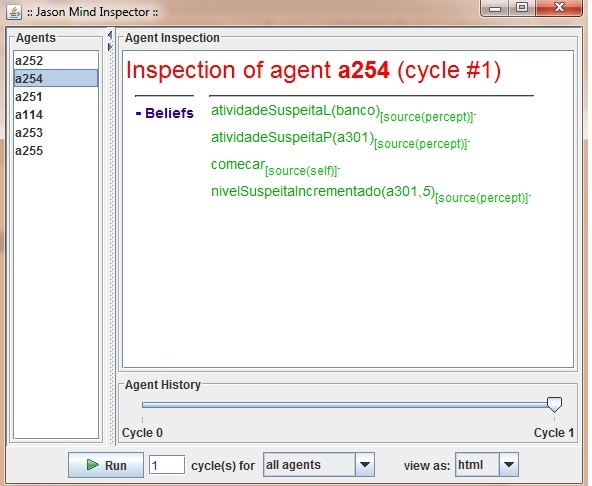
\includegraphics [height=10cm]{figuras/crencas_policial254.jpg}
\caption{Base de cranças do agente policial oculto a254}
\label{baseA254}
\end{figure}
\begin{figure}
\centering
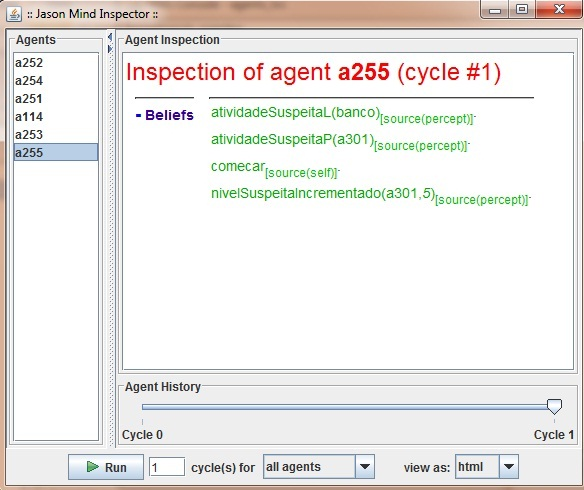
\includegraphics [height=10cm]{figuras/crencas_policial255.jpg}
\caption{Base de cranças do agente policial oculto a255}
\label{baseA255}
\end{figure}

